\documentclass{standalone}
\usepackage{standalone}

\begin{document}
\subsection{DNA Binding}
DNA-binding proteins are a specific type of proteins mainly composed of DNA-binding domains and thats why have a specific or general inclination for either single or double stranded DNA. That means in many cases those proteins are supposed to bind to a specific site or location of the DNA. This site of the DNA called a DNA-binding site. For example 
\begin{figure}[ht]
	\centering
	\fbox{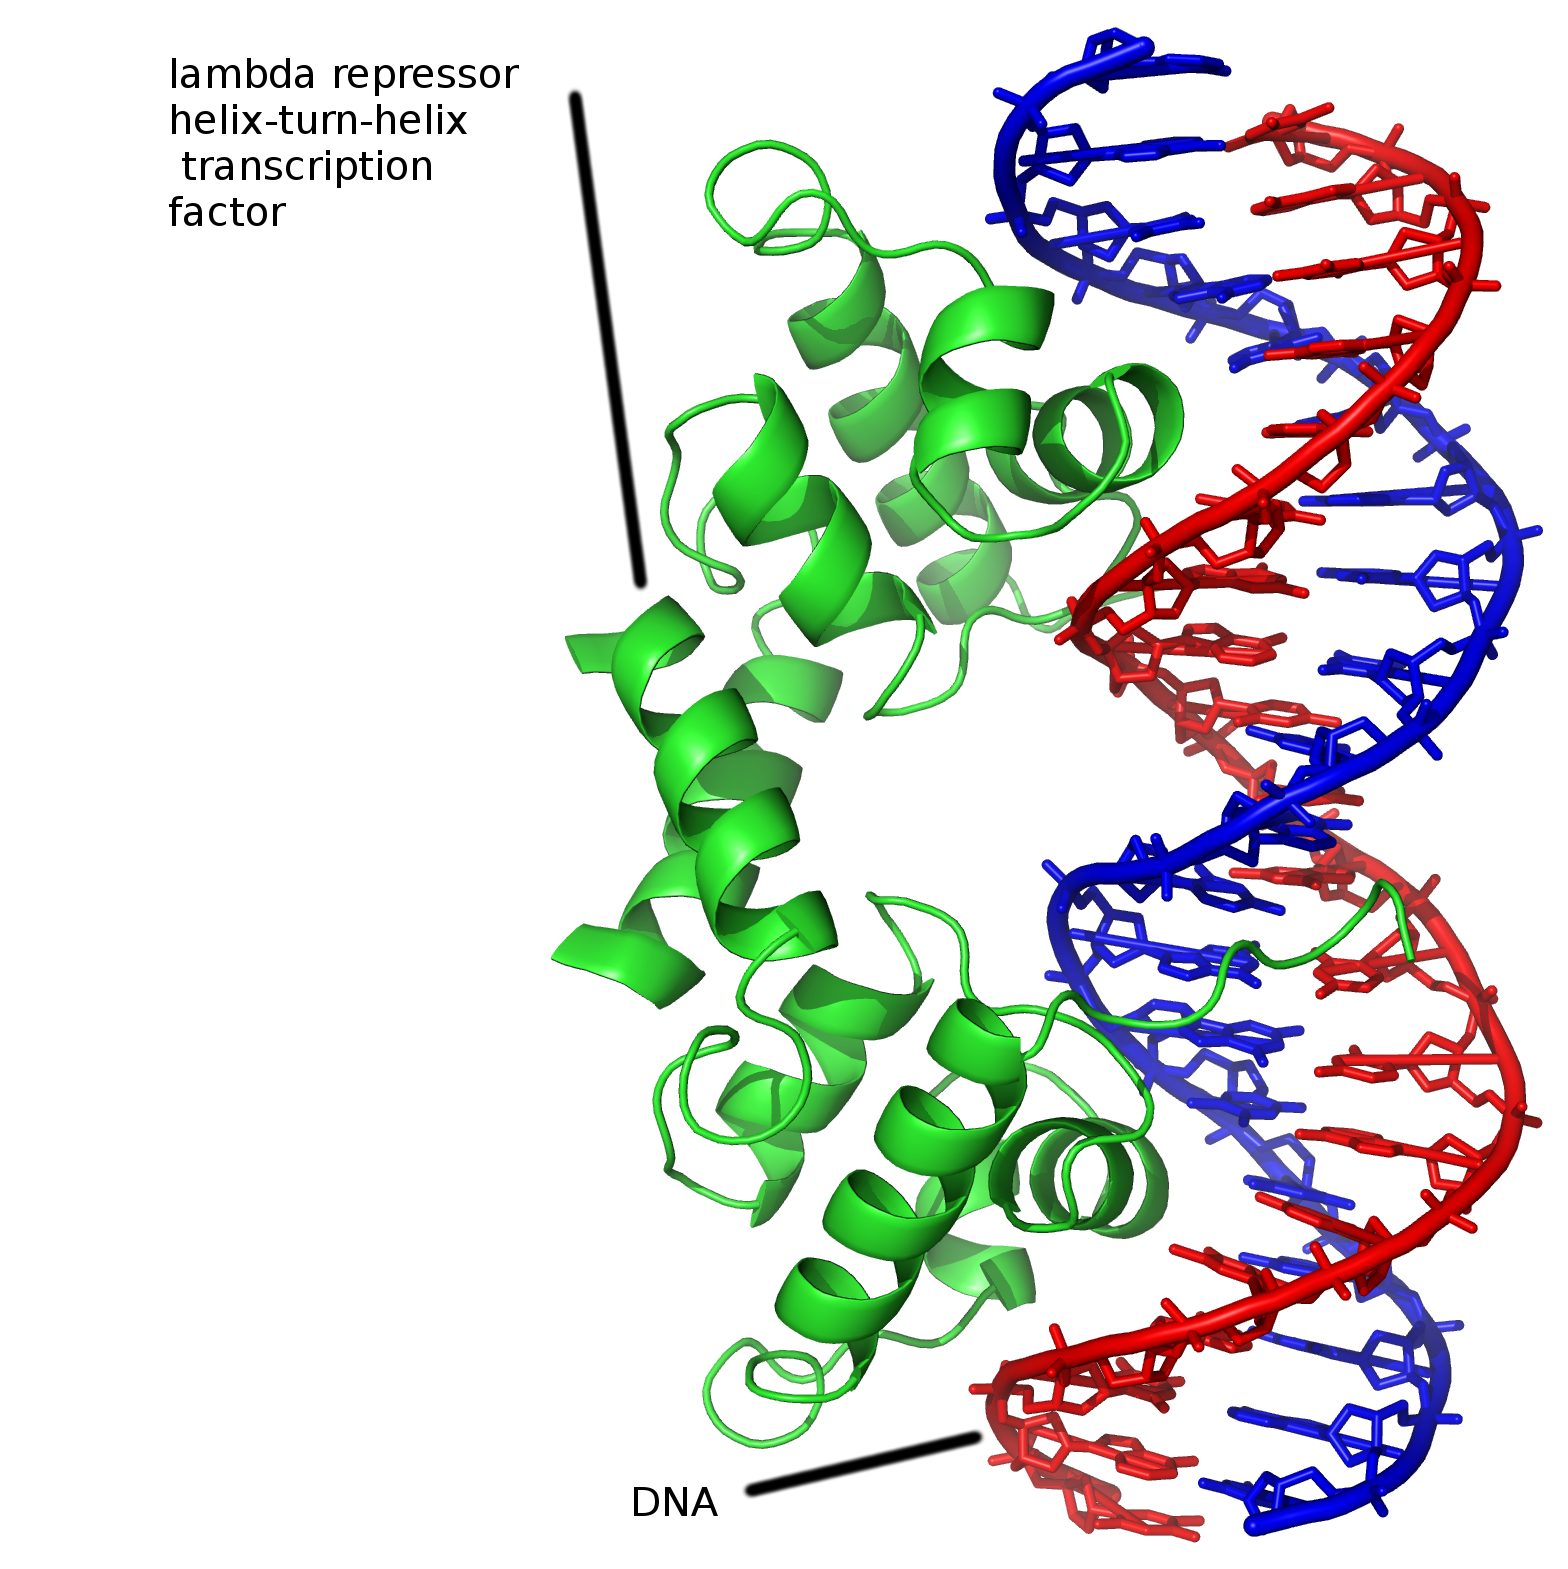
\includegraphics[scale=0.15]{./img/DNABinding3}}
	\caption{Picture of a lambda repressor helix-turn-helix transcription factor binding to its target location in DNA.}
	\label{fig:DNAB}
\end{figure}
\par 
In many cases locating these specific sites can be proven very important for may purposes. Like ChIP-sequencing\cite{dnaC} which used Solexa-sequencing\cite{dnaB} to find the locations of STAT1 sites in HeLa S3 cells\cite{dnaH}. Mapping longs reads rather than short ones to a large genome sequence obviously presents a algorithmic challenge.
\par 
Applications where such mapping and resequencing is being done a primary concern always remains how accurately it is done. So our goal is develop a mapping tool that can map reads to the reference accurately and consuming a feasible amount of time.
\end{document}